%%%%%%%%%%%%%%%%%%%%%%%%%%%%%%%%%%%%%%%%%
% Structured General Purpose Assignment
% LaTeX Template
%
% This template has been downloaded from:
% http://www.latextemplates.com
%
% Original author:
% Ted Pavlic (http://www.tedpavlic.com)
%
% Note:
% The \lipsum[#] commands throughout this template generate dummy text
% to fill the template out. These commands should all be removed when
% writing assignment content.
%
%%%%%%%%%%%%%%%%%%%%%%%%%%%%%%%%%%%%%%%%%

%----------------------------------------------------------------------------------------
%	PACKAGES AND OTHER DOCUMENT CONFIGURATIONS
%----------------------------------------------------------------------------------------

\documentclass{article}

\usepackage{fancyhdr} % Required for custom headers
\usepackage{lastpage} % Required to determine the last page for the footer
\usepackage{extramarks} % Required for headers and footers
\usepackage{graphicx} % Required to insert images
\usepackage{lipsum} % Used for inserting dummy 'Lorem ipsum' text into the template
\usepackage{enumerate}
\usepackage{booktabs}
\usepackage{amsmath}
\usepackage{booktabs}
\usepackage{multirow}
\usepackage[normalem]{ulem}
\useunder{\uline}{\ul}{}

% Margins
\topmargin=-0.45in
\evensidemargin=0in
\oddsidemargin=0in
\textwidth=6.5in
\textheight=9.0in
\headsep=0.25in

\linespread{1.5} % Line spacing

% Set up the header and footer
\pagestyle{fancy}
% \lhead{\hmwkAuthorName} % Top left header
\chead{\hmwkClass\ (\hmwkTitle)} % Top center header
%%\rhead{\firstxmark}
\rhead{} % Top right header
\lfoot{\lastxmark} % Bottom left footer
\cfoot{} % Bottom center footer
\rfoot{Page\ \thepage\ of\ \pageref{LastPage}} % Bottom right footer
\renewcommand\headrulewidth{0.4pt} % Size of the header rule
\renewcommand\footrulewidth{0.4pt} % Size of the footer rule

\setlength\parindent{0pt} % Removes all indentation from paragraphs

%----------------------------------------------------------------------------------------
%	DOCUMENT STRUCTURE COMMANDS
%	Skip this unless you know what you're doing
%----------------------------------------------------------------------------------------

% Header and footer for when a page split occurs within a problem environment
\newcommand{\enterProblemHeader}[1]{
\nobreak\extramarks{#1}{#1 continued on next page\ldots}\nobreak
\nobreak\extramarks{#1 (continued)}{#1 continued on next page\ldots}\nobreak
}

% Header and footer for when a page split occurs between problem environments
\newcommand{\exitProblemHeader}[1]{
\nobreak\extramarks{#1 (continued)}{#1 continued on next page\ldots}\nobreak
\nobreak\extramarks{#1}{}\nobreak
}

\setcounter{secnumdepth}{0} % Removes default section numbers
\newcounter{homeworkProblemCounter} % Creates a counter to keep track of the number of problems

\newcommand{\homeworkProblemName}{}
\newenvironment{homeworkProblem}[1][Question \arabic{homeworkProblemCounter}]{ % Makes a new environment called homeworkProblem which takes 1 argument (custom name) but the default is "Question #"
\stepcounter{homeworkProblemCounter} % Increase counter for number of problems
\renewcommand{\homeworkProblemName}{#1} % Assign \homeworkProblemName the name of the problem
\section{\homeworkProblemName} % Make a section in the document with the custom problem count
\enterProblemHeader{\homeworkProblemName} % Header and footer within the environment
}{
\exitProblemHeader{\homeworkProblemName} % Header and footer after the environment
}

\newcommand{\problemAnswer}[1]{ % Defines the problem answer command with the content as the only argument
\noindent\framebox[\columnwidth][c]{\begin{minipage}{0.98\columnwidth}#1\end{minipage}} % Makes the box around the problem answer and puts the content inside
}

\newcommand{\homeworkSectionName}{}
\newenvironment{homeworkSection}[1]{ % New environment for sections within homework problems, takes 1 argument - the name of the section
\renewcommand{\homeworkSectionName}{#1} % Assign \homeworkSectionName to the name of the section from the environment argument
\subsection{\homeworkSectionName} % Make a subsection with the custom name of the subsection
\enterProblemHeader{\homeworkProblemName\ [\homeworkSectionName]} % Header and footer within the environment
}{
\enterProblemHeader{\homeworkProblemName} % Header and footer after the environment
}

%----------------------------------------------------------------------------------------
%	EXPECTATION AND VARIANCE OPERATOR
%----------------------------------------------------------------------------------------
 \newcommand{\E}{\mathrm{E}}
 \newcommand{\Var}{\mathrm{Var}}
 \newcommand{\Cov}{\mathrm{Cov}}
 \newcommand{\Corr}{\mathrm{Corr}}

%----------------------------------------------------------------------------------------
%	NAME AND CLASS SECTION
%----------------------------------------------------------------------------------------

\newcommand{\hmwkTitle}{Case 5: Dupont Corporation} % Assignment title
\newcommand{\hmwkDueDate}{Tuesday,\ April\ 17,\ 2018} % Due date
\newcommand{\hmwkClass}{FIN\ 521} % Course/class
\newcommand{\hmwkClassTime}{2:00pm} % Class/lecture time
\newcommand{\hmwkAuthorName}{Wanbae Park, Sangwoo Park, Inhyuk Lee, Soyeon Chang} % Your name

%----------------------------------------------------------------------------------------
%	TITLE PAGE
%----------------------------------------------------------------------------------------

\title{
\vspace{2in}
\textmd{\textbf{\hmwkClass:\ \hmwkTitle}}\\
\normalsize\vspace{0.1in}\small{Due\ on\ \hmwkDueDate}\\
\vspace{3in}
}

\author{\textbf{\hmwkAuthorName}}
\date{} % Insert date here if you want it to appear below your name

%----------------------------------------------------------------------------------------

\begin{document}

\maketitle

%----------------------------------------------------------------------------------------
%	TABLE OF CONTENTS
%----------------------------------------------------------------------------------------

%\setcounter{tocdepth}{1} % Uncomment this line if you don't want subsections listed in the ToC

%%\newpage
%%\tableofcontents
\newpage

%----------------------------------------------------------------------------------------
%	Question 1
%----------------------------------------------------------------------------------------
\begin{homeworkProblem}
    From Kullman's view, the company needs transition of their business
    from a commodity chemical business to a specialty chemical and
    science-driven business, and DPC is no longer fit the strategic vision.
    Furthermore, expected growth rate of the division does not meet firm's
    target. It is the main reason why DuPont is considering a sale of the
    performance coating division. From the analysis by DuPont itself,
    it expects that annual growth of sales will be 3\% to 5\%, and growth of
    operating margin will be 10\% to 12\%.
\end{homeworkProblem}

%----------------------------------------------------------------------------------------
%	Question 2
%----------------------------------------------------------------------------------------
\begin{homeworkProblem}
    PE funds are more likely to buy DPC rather than strategic buyer.
    From the case, PE funds look for mature firms which do not require large
    capital expenditures or R\&D. Strategic firms wants to acquire firm which
    can make synergy with their original business. Considering industrial
    background and current status of DPC, PE funds are more likely to buy DPC
    because the industry is in steady state, therefore DPC does not need
    substantial capital or R\&D to expand their business.
\end{homeworkProblem}

%----------------------------------------------------------------------------------------
%	Question 3
%----------------------------------------------------------------------------------------
\begin{homeworkProblem}
    According to the case, the return drivers for a private equity are
    the use of leverage, growth in EBITDA, and multiple arbitrage.
    Leverage can reduce tax, and also help augment a sponsor's return.
    PE firms can get benefits from growth in EBITDA, they can raise EBITDA
    to the level of comparable companies by improving the target's operation.
    They also can get benefits from multiples by selling firms at higher multiple
    than which when buying it.
\end{homeworkProblem}

%----------------------------------------------------------------------------------------
%	Question 4
%----------------------------------------------------------------------------------------
\begin{homeworkProblem}
    \begin{enumerate}[a)]
        \item   %% a)
        If revenue growth is 5\% per year, and others are not changed,
        enterprise value will be increased to 4,116 because of increase
        in revenue.
        \item   %% b)
        In this case, because EBIT increases, enterprise value will also be
        increased to 4,859.
        \item   %% c)
        If terminal muitiple increases to 8.0x rather than 7.0x,
        terminal value increases from 6,207 to 7,032, therefore enterprise value
        increases to 5,345.
        \item   %% d)
        At first, the firm raises debt at $7.0 \times 372 = 2,604$ amount.
        Since the firm uses all available cash to pay down debt, the amount of
        free cash flow to equity will be zero because cash will be paid down
        debt, and therefore amount of debt and interest expense will decrease.
        If the firm raises debt, there will be interest tax shield, therefore
        enterprise value will be increased by the amount of tax shield.
        The amount of interest tax shield is 147(discounted at cost of debt),
        therefore enterprise value will be increased to 5,491.
        Table \ref{tab:prob4-is} and table \ref{tab:prob4-apv} shows the result of
        valuation after change variables. The underlined value is changed value.
        \begin{table}[ht]
\centering
\begin{tabular}{@{}cccccccc@{}}
\toprule
Metric                        &        & Closing & Projected    &              &              &              &              \\ \midrule
                              & 2011A  &         & 2012E        & 2013E        & 2014E        & 2015E        & 2016E        \\
Sales Growth (\%)             & 12.5\% &         & {\ul 5.0\%}  & {\ul 5.0\%}  & {\ul 5.0\%}  & {\ul 5.0\%}  & {\ul 5.0\%}  \\
Depreciation and Amortization & \$104  &         & \$115        & \$118        & \$122        & \$125        & \$130        \\
EBIT Margin (Pretax)          & 6.3\%  &         & {\ul 12.0\%} & {\ul 12.0\%} & {\ul 12.0\%} & {\ul 12.0\%} & {\ul 12.0\%} \\
Tax Rate                      & 25\%   &         & 25\%         & 25\%         & 25\%         & 25\%         & 25\%         \\
Capital Expenditures          & \$80   &         & \$115        & \$122        & \$132        & \$144        & \$150        \\
Net Working Capital (\%)      &        &         & 15\%         & 15\%         & 15\%         & 15\%         & 15\%         \\
Terminal EBITDA Multiple (x)  &        &         &              &              &              &              & {\ul 8.0}    \\
Cost of debt                  & 6.75\% &         &              &              &              &              &              \\
Unlevered Cost of Equity      & 11.2\% &         &              &              &              &              &              \\ \bottomrule
\end{tabular}
\caption{Stand-Alone Valuation of DPC}
\label{tab:prob4-is}
\end{table}

        \begin{table}[ht]
\centering
\begin{tabular}{@{}cccccccc@{}}
\toprule
                                & 2011A & Closing                 & 2012E       & 2013E       & 2014E       & 2015E       & 2016E       \\ \midrule
Net Sales                       & 4,281 &                         & {\ul 4,495} & {\ul 4,720} & {\ul 4,956} & {\ul 5,204} & {\ul 5,464} \\
Pretax Operating Income (EBIT)  & 268   &                         & {\ul 539}   & {\ul 566}   & {\ul 595}   & {\ul 624}   & {\ul 656}   \\
Interest Expense                &       &                         & (176)       & (160)       & (141)       & (122)       & (100)       \\
Earnings before Taxes           &       &                         & 364         & 407         & 453         & 503         & 556         \\
Taxes                           &       &                         & (91)        & (102)       & (113)       & (126)       & (139)       \\
Net Income                      &       &                         & 273         & 305         & 340         & 377         & 417         \\
                                &       &                         &             &             &             &             &             \\
Depreciation and Amortization   & 104   &                         & 115         & 118         & 122         & 125         & 130         \\
Increase in Net Working Capital &       &                         & (32)        & (34)        & (35)        & (37)        & (39)        \\
Capital Expenditures            &       &                         & (115)       & (122)       & (132)       & (144)       & (150)       \\
Free Cash Flow  (FCF)           &       &                         & 372         & 387         & 401         & 412         & 433         \\
EBITDA                          & 372   &                         & 654         & 684         & 717         & 749         & 786         \\
Terminal Value                  &       &                         &             &             &             &             & {\ul 6,599} \\
FCF, including TV               &       &                         & 372         & 387         & 401         & 412         & 7,032       \\
After tax interest expense      &       &                         & 132         & 120         & 106         & 91          & 75          \\
Change in Debt                  &       &                         & (241)       & (267)       & (295)       & (321)       & (1,481)     \\
Debt                            &       & {\ul 2,604}             & {\ul 2,363} & {\ul 2,096} & {\ul 1,801} & {\ul 1,481} & {\ul 0}     \\
Cash                            &       & {\ul 2,604}             & {\ul 2,604} & {\ul 2,604} & {\ul 2,604} & {\ul 2,604} & {\ul }      \\
Enterprise Value (EV)           &       & \textit{\textbf{5,345}} &             &             &             &             &             \\
Interest Tax Shield             &       &                         & 44          & 40          & 35          & 30          & 25          \\
PV Tax Shield                   &       & \textit{\textbf{147}}   &             &             &             &             &             \\
                                &       &                         &             &             &             &             &             \\
EV with Tax Shield              &       & \textit{\textbf{5,491}} &             &             &             &             &             \\ \bottomrule
\end{tabular}
\caption{APV analysis}
\label{tab:prob4-apv}
\end{table}

        \item   %% e)
        Table \ref{tab:prob4-changes} shows changes in enterprise value by
        changing metrics. It shows that enterprise value increases most after
        changing EBIT margin: 744, and the second largest driver was
        EBITDA multiple, which increases enterprise value by 485.
        Therefore, we can conclude that the key driver for increasing
        enterprise value is growth in EBITDA.
        \begin{table}[ht]
\centering
\begin{tabular}{@{}cc@{}}
\toprule
Metrics                  & Change in enterprise value \\ \midrule
Sales growth             & 146                        \\
EBIT margin              & 744                        \\
Terminal EBITDA multiple & 485                        \\
Debt                     & 147                        \\ \bottomrule
\end{tabular}
\caption{Changes of enterprise value by changing metrics}
\label{tab:prob4-changes}
\end{table}

    \end{enumerate}
\end{homeworkProblem}

%----------------------------------------------------------------------------------------
%	Question 5
%----------------------------------------------------------------------------------------
\begin{homeworkProblem}
    If the buyers do not change anything, they will get zero return
    because enterprise value of the firm will never change,
    therefore they cannot get any positive return from the firm value.
    Furthremore since buyers do not use leverage, they don't have to pay
    any interest, therefore their return will be zero.
\end{homeworkProblem}

%----------------------------------------------------------------------------------------
%	Question 6
%----------------------------------------------------------------------------------------
\begin{homeworkProblem}
    \begin{enumerate}[a)]
        \item   %% a)
        From question 5-d, the PE fund raises debt by 2,604 million dollars.
        Therefore, if it buys DPC of 4.5 billion dollars, the amount of equity
        required is $4,500 - 2,604 = 1,896$ million dollars.
        \item   %% b)
        Since the firm uses all available cash to pay down debt, we assumed that
        there is no dividend paid out from 2012 to 2016.
        Assuming this, enterprise value at 2016 is calcualated as 7,032,
        which includes terminal value of free cash flows, and there is 1,481
        amount of remaining debt, and 75 amount of after tax expense. Therefore,
        cash flow for calculating IRR is $7,032 - 1,481 - 75 = 5,476$.
        Since there is 1,896 amount of equity investment at initial period and
        no intermediate cash flows, IRR is calculated as about 24\%.
        \item   %% c)
        Assuming the amount of debt is same as 2,604 million dollars, and set
        IRR at fixed amount of 20\%, we calculated maximum enterprise value
        by using Excel Goal Seek function. From the result, the maximum amount
        of available payment is about 2,200.23 million dollars, therefore adding
        up with the amount of debt, maximum enterprise value of the firm is
        calculated as $2,604 + 2,200.23 = 4,804.22$.
        \item   %% d)
        By changing the amount of debt from $EBITDA \times i$, where $i = 1, 2, 3
        \dots 10$, we calculated IRR, and Figure \ref{fig:irr} shows the
        relationship between IRR and the amount of equity invested.
        \begin{figure}[ht]
            \centering
            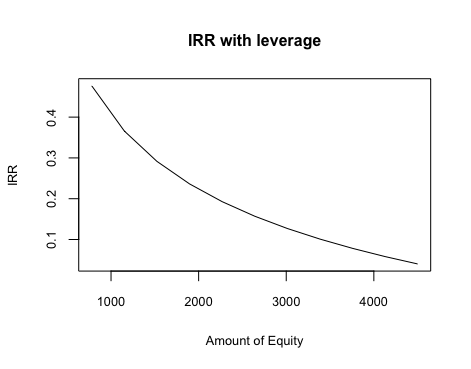
\includegraphics[scale = 0.6]{irr.png}
            \caption{IRR against the amount of equity invested}
            \label{fig:irr}
        \end{figure}
        From the plot, we can discover that IRR decreases as the amount of
        equity invested increases. It justifies the needs of debt financing
        when acquiring a firm.
        Furthermore, assuming PE firm cannot use leverage, we calculated maximum
        enterprise value a fund can pay for remaining IRR as 20\% using the same
        method in c). It was calculated as 3,831.675, which is lower than result
        from c). It also justifies needs for debt financing.
        \item   %% e)
        There is some advantages using debt for buying firms.
        First, it can reduce costs of capital benefiting from interest tax shield.
        Second, it can raise opportunities of acquiring large firm with fixed
        IRR. From c), and d), we discovered that the maximum enterprise value
        the firm can pay for increases when using debt.
        However, there is also some disadvantages for using debt.
        The major disadvantage is increase in cost of equity, which increases
        risk of the investment including failure to paying out debt.
        Another disadvantage is proportion of ownership. If the firm uses debt
        their proportion of ownership will decrease.
    \end{enumerate}
\end{homeworkProblem}

%----------------------------------------------------------------------------------------
%	Question 7
%----------------------------------------------------------------------------------------
\begin{homeworkProblem}
    DuPont sold DPC to Carlyle, which is one of the private equity's top investors.
    The selling price was \$4.9 billion, and after purchase, EBITDA
    increased by about 20\%. Consequently net income increased
    about 3.2\%. From the newpaper article at 2016, its enterprise value
    increased to 9.6 billion dollars. Carlyle finally shed its stake at 2016,
    and its annualized total return from its investor is 80\%. It cleared
    its position by 6 ways, including IPO and Berkshire Hathaway deal.
\end{homeworkProblem}
\end{document}
